\section{\textit{Transformer}}

\textit{Transformer} telah mengubah lanskap pemrosesan bahasa alami (NLP) dengan cara yang signifikan. Dalam makalah mereka, penulis memperkenalkan konsep baru yang disebut mekanisme \textit{self-attention} \parencite{transformers}. Mekanisme ini memungkinkan setiap kata dalam input untuk memfokuskan pada kata-kata lain dalam sekuens yang sama, memberikan model kemampuan untuk memahami konteks dengan lebih baik. Ini berbeda dari pendekatan sebelumnya yang biasanya mengandalkan informasi lokal atau posisi tetap dalam sekuens.

\begin{figure}[ht]
    \centering
    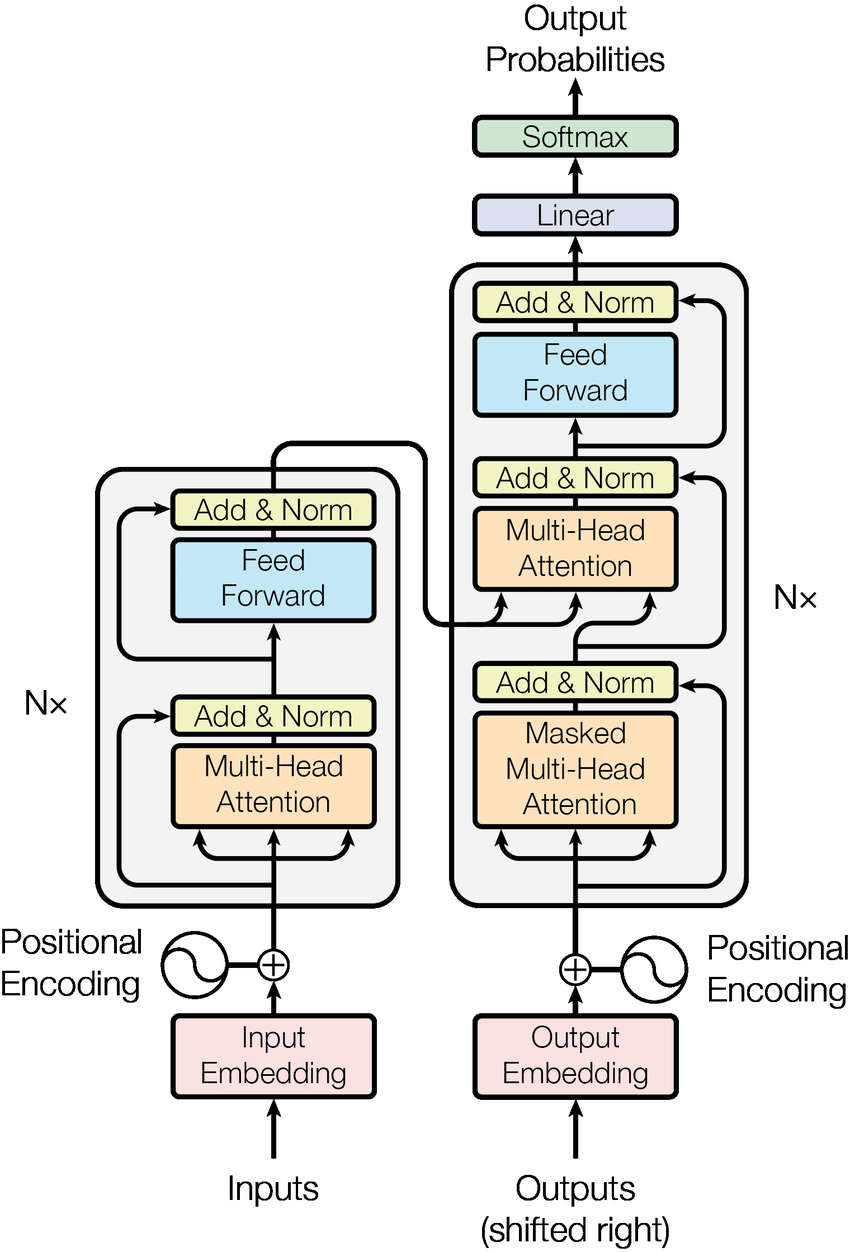
\includegraphics[width=0.8\textwidth]{chapter-2/transformer.png}
    \caption{Arsitektur \textit{Transformer} \parencite{transformers}}
    \label{fig:transformer}
\end{figure}

Salah satu keunggulan utama dari mekanisme \textit{self-attention} adalah kemampuannya untuk menangani sekuens dengan panjang yang berbeda dan memahami hubungan antar kata tanpa mempertimbangkan jarak antara mereka. Ini memungkinkan Transformer untuk memahami ketergantungan jarak jauh dalam teks, sesuatu yang sulit dicapai oleh arsitektur sebelumnya seperti RNN dan LSTM.

Selain itu, Transformer dirancang untuk paralelisasi, yang memungkinkannya dilatih dengan cepat pada perangkat keras modern. Ini mempercepat penelitian dan pengembangan dalam NLP dan memungkinkan \textit{training} model skala besar seperti BERT dan GPT yang sekarang mendominasi bidang ini.

Sejak diperkenalkannya Transformer, banyak variasi dan peningkatan telah dikembangkan. Namun, prinsip dasar \textit{self-attention} dan paralelisasi yang diperkenalkan oleh Transformer tetap menjadi inti dari banyak inovasi dalam NLP kontemporer.